% Options for packages loaded elsewhere
% Options for packages loaded elsewhere
\PassOptionsToPackage{unicode}{hyperref}
\PassOptionsToPackage{hyphens}{url}
\PassOptionsToPackage{dvipsnames,svgnames,x11names}{xcolor}
%
\documentclass[
  british,
  a4paper,
]{article}
\usepackage{xcolor}
\usepackage{amsmath,amssymb}
\setcounter{secnumdepth}{-\maxdimen} % remove section numbering
\usepackage{iftex}
\ifPDFTeX
  \usepackage[T1]{fontenc}
  \usepackage[utf8]{inputenc}
  \usepackage{textcomp} % provide euro and other symbols
\else % if luatex or xetex
  \usepackage{unicode-math} % this also loads fontspec
  \defaultfontfeatures{Scale=MatchLowercase}
  \defaultfontfeatures[\rmfamily]{Ligatures=TeX,Scale=1}
\fi
\usepackage{lmodern}
\ifPDFTeX\else
  % xetex/luatex font selection
\fi
% Use upquote if available, for straight quotes in verbatim environments
\IfFileExists{upquote.sty}{\usepackage{upquote}}{}
\IfFileExists{microtype.sty}{% use microtype if available
  \usepackage[]{microtype}
  \UseMicrotypeSet[protrusion]{basicmath} % disable protrusion for tt fonts
}{}
\makeatletter
\@ifundefined{KOMAClassName}{% if non-KOMA class
  \IfFileExists{parskip.sty}{%
    \usepackage{parskip}
  }{% else
    \setlength{\parindent}{0pt}
    \setlength{\parskip}{6pt plus 2pt minus 1pt}}
}{% if KOMA class
  \KOMAoptions{parskip=half}}
\makeatother
% Make \paragraph and \subparagraph free-standing
\makeatletter
\ifx\paragraph\undefined\else
  \let\oldparagraph\paragraph
  \renewcommand{\paragraph}{
    \@ifstar
      \xxxParagraphStar
      \xxxParagraphNoStar
  }
  \newcommand{\xxxParagraphStar}[1]{\oldparagraph*{#1}\mbox{}}
  \newcommand{\xxxParagraphNoStar}[1]{\oldparagraph{#1}\mbox{}}
\fi
\ifx\subparagraph\undefined\else
  \let\oldsubparagraph\subparagraph
  \renewcommand{\subparagraph}{
    \@ifstar
      \xxxSubParagraphStar
      \xxxSubParagraphNoStar
  }
  \newcommand{\xxxSubParagraphStar}[1]{\oldsubparagraph*{#1}\mbox{}}
  \newcommand{\xxxSubParagraphNoStar}[1]{\oldsubparagraph{#1}\mbox{}}
\fi
\makeatother


\usepackage{longtable,booktabs,array}
\newcounter{none} % for unnumbered tables
\usepackage{calc} % for calculating minipage widths
% Correct order of tables after \paragraph or \subparagraph
\usepackage{etoolbox}
\makeatletter
\patchcmd\longtable{\par}{\if@noskipsec\mbox{}\fi\par}{}{}
\makeatother
% Allow footnotes in longtable head/foot
\IfFileExists{footnotehyper.sty}{\usepackage{footnotehyper}}{\usepackage{footnote}}
\makesavenoteenv{longtable}
\usepackage{graphicx}
\makeatletter
\newsavebox\pandoc@box
\newcommand*\pandocbounded[1]{% scales image to fit in text height/width
  \sbox\pandoc@box{#1}%
  \Gscale@div\@tempa{\textheight}{\dimexpr\ht\pandoc@box+\dp\pandoc@box\relax}%
  \Gscale@div\@tempb{\linewidth}{\wd\pandoc@box}%
  \ifdim\@tempb\p@<\@tempa\p@\let\@tempa\@tempb\fi% select the smaller of both
  \ifdim\@tempa\p@<\p@\scalebox{\@tempa}{\usebox\pandoc@box}%
  \else\usebox{\pandoc@box}%
  \fi%
}
% Set default figure placement to htbp
\def\fps@figure{htbp}
\makeatother



\ifLuaTeX
\usepackage[bidi=basic,shorthands=off]{babel}
\else
\usepackage[bidi=default,shorthands=off]{babel}
\fi
\ifLuaTeX
  \usepackage{selnolig} % disable illegal ligatures
\fi


\setlength{\emergencystretch}{3em} % prevent overfull lines

\providecommand{\tightlist}{%
  \setlength{\itemsep}{0pt}\setlength{\parskip}{0pt}}



 


\makeatletter
\@ifpackageloaded{tcolorbox}{}{\usepackage[skins,breakable]{tcolorbox}}
\@ifpackageloaded{fontawesome5}{}{\usepackage{fontawesome5}}
\definecolor{quarto-callout-color}{HTML}{909090}
\definecolor{quarto-callout-note-color}{HTML}{0758E5}
\definecolor{quarto-callout-important-color}{HTML}{CC1914}
\definecolor{quarto-callout-warning-color}{HTML}{EB9113}
\definecolor{quarto-callout-tip-color}{HTML}{00A047}
\definecolor{quarto-callout-caution-color}{HTML}{FC5300}
\definecolor{quarto-callout-color-frame}{HTML}{acacac}
\definecolor{quarto-callout-note-color-frame}{HTML}{4582ec}
\definecolor{quarto-callout-important-color-frame}{HTML}{d9534f}
\definecolor{quarto-callout-warning-color-frame}{HTML}{f0ad4e}
\definecolor{quarto-callout-tip-color-frame}{HTML}{02b875}
\definecolor{quarto-callout-caution-color-frame}{HTML}{fd7e14}
\makeatother
\makeatletter
\@ifpackageloaded{caption}{}{\usepackage{caption}}
\AtBeginDocument{%
\ifdefined\contentsname
  \renewcommand*\contentsname{Table of contents}
\else
  \newcommand\contentsname{Table of contents}
\fi
\ifdefined\listfigurename
  \renewcommand*\listfigurename{List of Figures}
\else
  \newcommand\listfigurename{List of Figures}
\fi
\ifdefined\listtablename
  \renewcommand*\listtablename{List of Tables}
\else
  \newcommand\listtablename{List of Tables}
\fi
\ifdefined\figurename
  \renewcommand*\figurename{Figure}
\else
  \newcommand\figurename{Figure}
\fi
\ifdefined\tablename
  \renewcommand*\tablename{Table}
\else
  \newcommand\tablename{Table}
\fi
}
\@ifpackageloaded{float}{}{\usepackage{float}}
\floatstyle{ruled}
\@ifundefined{c@chapter}{\newfloat{codelisting}{h}{lop}}{\newfloat{codelisting}{h}{lop}[chapter]}
\floatname{codelisting}{Listing}
\newcommand*\listoflistings{\listof{codelisting}{List of Listings}}
\makeatother
\makeatletter
\makeatother
\makeatletter
\@ifpackageloaded{caption}{}{\usepackage{caption}}
\@ifpackageloaded{subcaption}{}{\usepackage{subcaption}}
\makeatother
\usepackage{bookmark}
\IfFileExists{xurl.sty}{\usepackage{xurl}}{} % add URL line breaks if available
\urlstyle{same}
% fallback for those not using the hyperref driver hyperxmp:
\makeatletter
\@ifundefined{xmpquote}{\newcommand{\xmpquote}[1]{#1}}{}
\makeatother
\hypersetup{
  pdftitle={Global macro monitoring and external-debt vulnerability},
  pdfauthor={Carlos Galindo},
  pdflang={en-GB},
  colorlinks=true,
  linkcolor={blue},
  filecolor={Maroon},
  citecolor={Blue},
  urlcolor={Blue},
  pdfcreator={LaTeX via pandoc}}


\title{Global macro monitoring and external-debt vulnerability}
\usepackage{etoolbox}
\makeatletter
\providecommand{\subtitle}[1]{% add subtitle to \maketitle
  \apptocmd{\@title}{\par {\large #1 \par}}{}{}
}
\makeatother
\subtitle{A repeatable way to turn a week's data flow into a causal read
of inflation, policy and external risk}
\author{Carlos Galindo}
\date{}
\begin{document}
\maketitle


\begin{tcolorbox}[enhanced jigsaw, arc=.35mm, bottomrule=.15mm, breakable, colback=white, colframe=quarto-callout-note-color-frame, left=2mm, leftrule=.75mm, opacityback=0, rightrule=.15mm, toprule=.15mm]

\vspace{-3mm}\textbf{At a glance}\vspace{3mm}

\begin{itemize}
\tightlist
\item
  \textbf{Question.} How can one person keep a disciplined, comparable
  read on inflation and central-bank behaviour across a dozen economies,
  and judge which emerging markets are exposed on external debt?
\item
  \textbf{Approach.} Short notes built on one template: separate the
  forces acting on prices and policy, say which way each pushes, and
  name what would change the call. For external debt, a layered
  indicator framework that groups measures by the channel through which
  they hurt.
\item
  \textbf{Finding.} The same few channels recur across very different
  economies, and a policy decision is best explained by weighing several
  forces, not by one headline. External vulnerability shows up where
  thin reserves, short maturities and a weak current account coincide.
\item
  \textbf{Why it matters.} A consistent structure makes cross-country
  comparison fast, makes the reasoning checkable, and keeps analysis
  going between jobs.
\end{itemize}

\end{tcolorbox}

\subsection{The question}\label{the-question}

After leaving a research role in June 2024, I kept up a daily habit of
global macro monitoring through to September 2024. The aim was
practical. Each week brings inflation prints, central-bank decisions and
market moves in many countries, and the risk for any analyst is a pile
of unconnected comments. A note on one country can be convincing and
still be impossible to compare with the note on the next.

Two questions shaped the work. First, for inflation and monetary policy,
what is the short list of forces that decide where a central bank goes
next, and can the same list be applied to a dozen economies without
losing what is specific to each? Second, for emerging markets, how
should one judge external-debt vulnerability when the standard
indicators disagree, as they often do? A country with a high
debt-to-exports ratio but deep reserves is in a different position from
one with a modest ratio and almost no buffer.

The obvious approach, a paragraph of commentary per country, falls short
in both cases. It hides the weights the author is implicitly using, and
it cannot show a reader what would change the conclusion.

\subsection{Approach}\label{approach}

\textbf{Short country notes.} Each note follows the same logic. It
starts from the policy decision or the inflation outcome to be
explained. It then lists the forces acting on it, grouped as external
(global disinflation, the stance of larger central banks, commodity
prices), domestic demand and supply (labour-market tightness, public
spending, administered prices such as electricity tariffs, credit
conditions), and the policy reaction itself. Every force is given a
direction, and the feedback from the policy decision back onto demand or
communication is marked separately, because a rate cut that revives
demand changes the next decision. Each note ends with the ``swing
factor'': the single development that would flip the call.

The notes covered inflation and policy in a dozen economies, spanning
central and eastern Europe, the Middle East and Africa, Latin America,
Asia and Australia. Where a country had a clear divergence from its
peers, for example upside inflation surprises in a few high-inflation
economies against downside surprises elsewhere, the note was written to
explain the divergence and not just report it.

\textbf{External-debt vulnerability.} The framework groups indicators by
channel instead of presenting a long flat list. I settled on five
families: debt burden and structure; reserve cover; wider financial
fragility; macroeconomic and external conditions; and institutional and
structural features. Within debt, the measures are debt relative to
exports, debt service relative to exports and to government revenue, the
share of debt in foreign currency, and average maturity. Reserve cover
is read against short-term debt, against broad money and in months of
imports. Financial fragility adds the share of short-term debt, bank
loan quality and capital, and household debt. The macro family covers
the current account, the net international investment position, external
financing needs, exchange-rate behaviour and terms of trade. The
structural family covers openness, fiscal balance, policy credibility
and dependence on commodities, tourism or remittances.

A second pass turned the list into a causal map. The current account
feeds debt service and the risk of a sudden stop; terms-of-trade and
exchange-rate volatility feed the current account; global risk appetite
feeds both sudden stops and exchange-rate volatility; maturity structure
feeds refinancing risk. The point of the map is to say which indicators
are inputs and which are consequences, so that two high readings that
share one cause are not counted twice.

\textbf{Checking.} The template builds in three tests: do the forces
named actually explain the outcome that was observed; does the direction
attached to each force survive a plain reading of the data release; and
does the swing factor correspond to something observable soon. A call
that cannot be falsified soon is not a call. Survey-based market
expectations were used only as summary findings from Bloomberg survey
data (2024), never reproduced.

\subsection{What the work shows}\label{what-the-work-shows}

\textbf{Policy is a weighing exercise.} In the Latin American and
central European cases, central-bank decisions were best explained by a
balance of forces pulling in different directions. In one example,
strong domestic demand, higher commodity prices and administered-price
increases pushed inflation up, while global disinflation and softer
private credit pulled the other way. The outcome was a cautious move
paired with firm communication, and the real information was in the
signal about the pace of future moves. A note that reported only the
decision would have missed this.

\textbf{Divergence has identifiable causes.} Across the emerging
economies of central and eastern Europe, the Middle East and Africa,
lower commodity prices and favourable base effects produced disinflation
in most economies, while overheating from loose fiscal policy and strong
domestic demand explained upside surprises in a small group. The usual
grouping by region was less useful than grouping by cause.

\textbf{Labour-market stories need the other side.} In a
developed-market example, a tight labour market, driven by public-sector
and care-sector expansion, immigration and rising participation, pressed
wages and prices upward. The note also recorded the counter-scenario,
that firms may be holding on to workers, so that unemployment could rise
faster than forecasts suggest once higher rates bite. Keeping both in
view is what stopped the note from becoming a one-sided story.

The first figure shows what this kind of decomposition looks like in a
form that can be compared across countries. It is simulated, but it has
the structure of the notes: a dozen economies, a handful of forces, and
a signed contribution from each.

\begin{figure}

\centering{

\pandocbounded{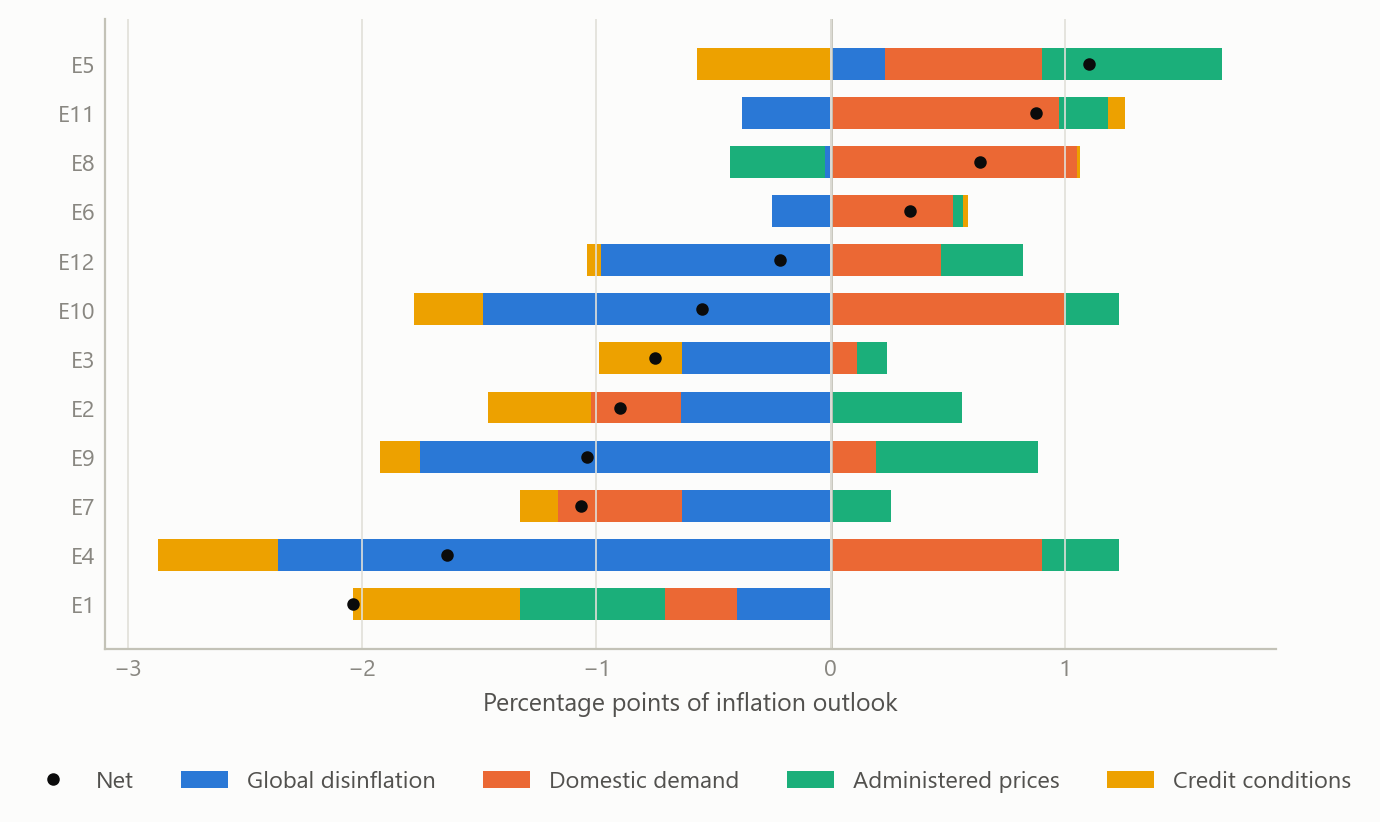
\includegraphics[keepaspectratio]{index_files/figure-latex/fig-forces-output-1.png}}

}

\caption{\label{fig-forces}Signed contribution of four forces to the
inflation outlook, twelve economies (simulated data).}

\end{figure}%

\textbf{External vulnerability is about coincidence.} No single
indicator separated the fragile cases from the resilient ones in the
framework. What mattered was the overlap of three conditions: reserves
that are thin relative to short-term debt, a large share of debt falling
due soon or denominated in foreign currency, and a current account that
depends on volatile export earnings. Where these coincide, a change in
global risk appetite is enough to turn a manageable position into a
financing problem. Where only one is present, the position is usually
absorbable.

The second figure illustrates the screening logic with simulated
emerging markets: reserve cover plotted against short-term debt
exposure, with the group flagged when the third condition also holds.

\begin{figure}

\centering{

\pandocbounded{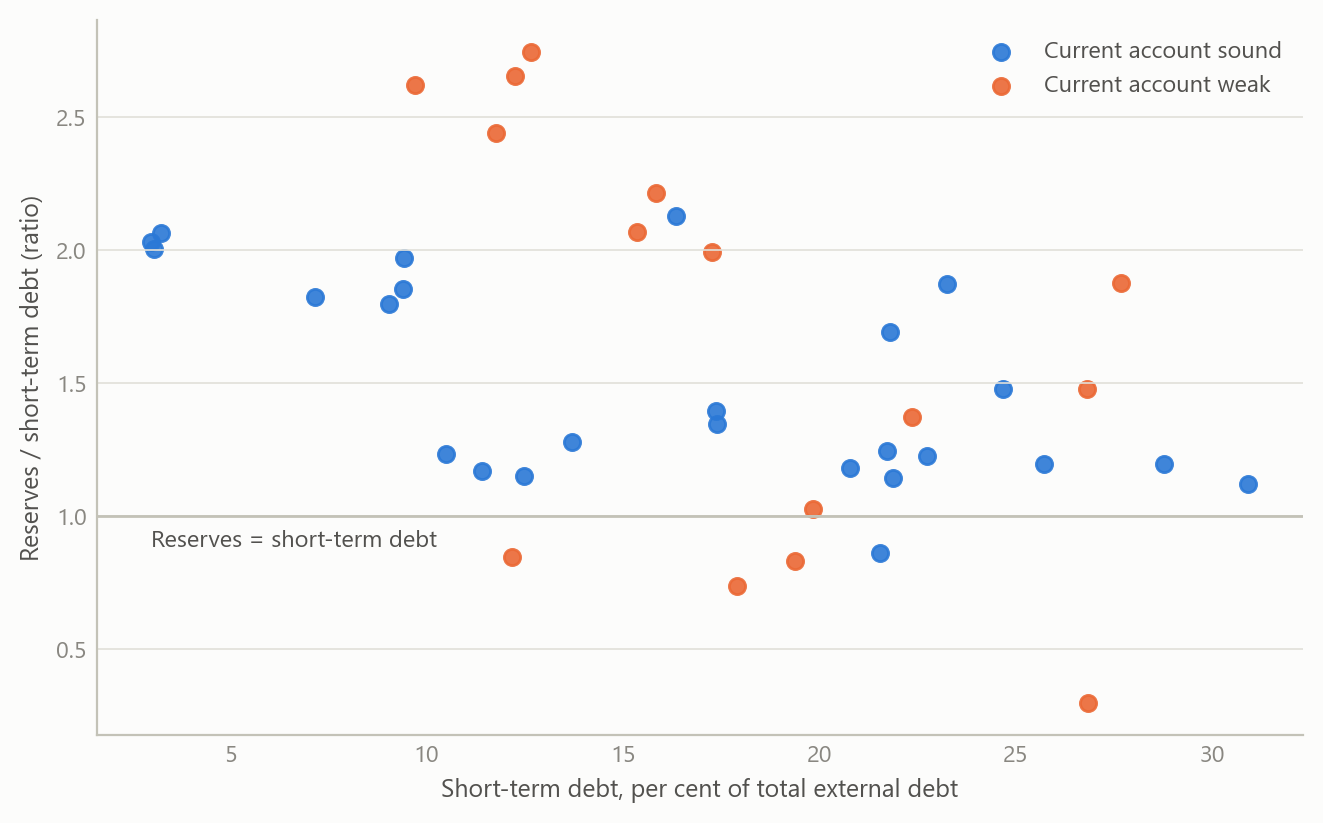
\includegraphics[keepaspectratio]{index_files/figure-latex/fig-screen-output-1.png}}

}

\caption{\label{fig-screen}Reserve cover against short-term debt share
for 40 emerging markets; flagged where the current account is also weak
(simulated data).}

\end{figure}%

The layered structure also gave a way to rank countries by channel. The
third figure shows a simple composite in which each family contributes
to a score, so a reader can see not only who ranks highest but why.

\begin{figure}

\centering{

\pandocbounded{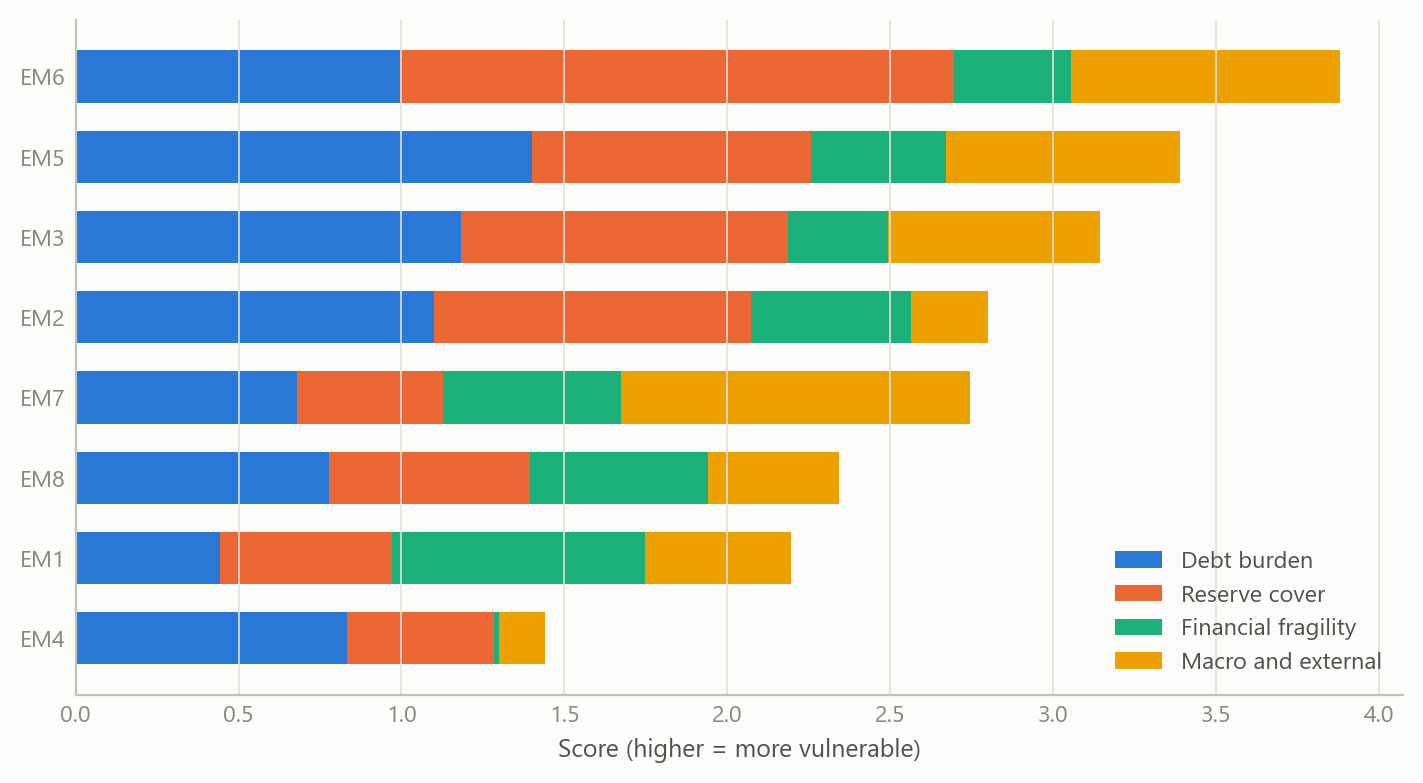
\includegraphics[keepaspectratio]{index_files/figure-latex/fig-composite-output-1.png}}

}

\caption{\label{fig-composite}Composite external-vulnerability score by
family for eight emerging markets (simulated data).}

\end{figure}%

\subsection{Insights}\label{insights}

\begin{enumerate}
\def\labelenumi{\arabic{enumi}.}
\tightlist
\item
  \textbf{Weights should be visible.} A note that lists forces with
  signs lets a reader disagree with one weight without rejecting the
  whole view. That is the main reason the template mattered more than
  any individual call.
\item
  \textbf{Communication is part of the decision.} Several central banks
  paired a move with a firm signal. The forecastable part was often the
  pace of what comes next, not the move itself.
\item
  \textbf{Group by cause, not by region.} Disinflation and its
  exceptions lined up with commodity prices, base effects and fiscal
  stance far better than with geography.
\item
  \textbf{Indicators are not independent.} Mapping which measures are
  inputs and which are outcomes prevents double-counting and shows where
  one shock would register in several measures at once.
\item
  \textbf{Write down the swing factor.} Naming what would change the
  view turns commentary into a testable statement and makes the next
  update easier.
\end{enumerate}

\subsection{Scope and next steps}\label{scope-and-next-steps}

The monitoring framework is built for fast, falsifiable calls:
indicators grouped by channel into five families, each call tied to a
swing factor that can be observed soon, and the reasoning behind each
call written down so it can be checked against what followed.

The natural extensions are two. First, calibration on a panel of past
episodes, estimating how much each family adds to the probability of
financing stress and whether the joint signal of thin reserves, short
maturities and a weak current account beats any single indicator.
Second, testing the cross-country decomposition against subsequent
policy decisions, to measure the predictive value of its signs and swing
factors.

The maps and notes behind individual calls can be discussed on request.

\subsection{About the evidence}\label{about-the-evidence}

The work is real: June to September 2024, covering inflation and
monetary policy in about a dozen economies and a framework for
external-debt vulnerability in emerging markets, produced as short notes
and causal maps. Market-survey inputs were used only as summary findings
from Bloomberg survey data (2024). Everything shown as a figure on this
page is illustrative and generated for this page.

Figures and tables marked \emph{simulated} are generated from simulated
data built to share the structure of the analysis (its variables,
horizons and frequencies). They show how each method works and what its
output looks like. Results stated in the text, and figures that give a
source, are the project's own. Methods are described at the level of a
methods section. Code and data pipelines are not reproduced here.




\end{document}
